\documentclass[12pt,a4paper]{article}
\usepackage[utf8]{inputenc}
\usepackage{amsmath,amsthm, amssymb}
\usepackage{amsfonts}
\usepackage{amssymb}
\usepackage{graphicx} % For pictures
\usepackage[export]{adjustbox}
\usepackage{pdfpages} % for pdfs
\usepackage{listings}
\usepackage{xcolor}
\usepackage{caption}

\definecolor{mGreen}{rgb}{0,0.6,0}
\definecolor{mGray}{rgb}{0.5,0.5,0.5}
\definecolor{mPurple}{rgb}{0.58,0,0.82}
\definecolor{backgroundColour}{rgb}{0.95,0.95,0.95}

\lstdefinestyle{CStyle}{
	backgroundcolor=\color{backgroundColour},   
	commentstyle=\color{mGreen},
	keywordstyle=\color{magenta},
	numberstyle=\tiny\color{mGray},
	stringstyle=\color{mPurple},
	basicstyle=\footnotesize,
	breakatwhitespace=false,         
	breaklines=true,                 
	captionpos=b,                    
	keepspaces=true,                 
	numbers=left,                    
	numbersep=5pt,                  
	showspaces=false,                
	showstringspaces=false,
	showtabs=false,                  
	tabsize=2,
	language=C
}
\lstset{style=CStyle}
\usepackage{titling}
\usepackage[margin=0.75in]{geometry}
\setlength{\droptitle}{-7em}   % This is your set screw
\date{}
\setlength{\parindent}{0em}

\author{Lara Quitte, Tino Jeromin}
\title{Versuch 1: Buffer Overflow}


\begin{document}
	\maketitle
	
	
	\section*{Hintergrundwissen}
	Ein Programm in C ist in folgende Speicherbereiche aufgeteilt:
	\begin{itemize}
		\item Stack
		\item Heap
		\item Uninitialized data
		\item Initialized data 
		\item Text
	\end{itemize}
	
	Diese Bereiche sollen im Folgenden kurz näher betrachtet werden. Ausserdem soll ein Buffer-Overflow sowie Stack- und Heap-Overflow erläutert werden.
	\bigskip
	
	\textbf{Heap} \\
	Der Heap wird in C genutzt, um dynamisch Speicher für Variablen, Arrays, etc zu reservieren.
	Es wird also während der Laufzeit des Programms Speicher reserviert und wieder freigegeben.
	Dies geschieht mittels 'malloc', 'realloc' und 'calloc'. 
	Die so angelegten Variablen und ihr Speicherplatz existieren bis sie vom Programm mittels 'free' wieder
	freigegeben werden. Werden die angelegten Variablen nicht wieder freigegeben, kann es zu Memory Leaks
	kommen, d. h. das Programm reserviert immer mehr Speicher, gibt ihn aber nicht wieder frei, bis kein 
	Speicherplatz mehr verfügbar ist.
	\bigskip
	
	\textbf{Stack} \\
	Auf dem Stack werden die Funktionen und die dazugehörigen Informationen gespeichert.
	Ruft also ein Programm eine Funktion auf, wird die Rücksprungadresse, die übergebenen Parameter und 
	alle lokalen Variablen auf den Stack gelegt. Diese Informationen werden zusammen Stack Frame genannt, 
	was jede Funktion besitzt.
	Ist eine Funktion beendet, wird der Stack Frame wieder vom Stack genommen und das Programm springt 
	zu der Funktion, die diese Funktion aufgerufen hat.
	Das Legen einer Variable auf den Stack wird als 'push' bezeichnet und das entfernen vom Stack als 'pop'.
	Das Betriebssystem speichert typischerweise mittels eines Zeigers den Anfang des Stacks und das aktuell 
	oberste Element des Stacks.
	Der Stack ist je nach Betriebssystem und CPU unterschiedlich implementiert.
	\bigskip
	
	\textbf{Uninitialized data}\\
	Hier werden alle globalen und statischen Variablen gespeichert, welche nicht initialisiert wurden, oder 
	zu 0 initialisiert wurden.
	\bigskip
	
	\textbf{Initialized data}\\
	Hier werden alle globalen und statischen Variablen gespeichert, welche vom Programmierer initialisiert 
	wurden. 
	Zusätzlich gibt es einen Bereich für read-write Zugriff und einen für read-only Zugriff.
	\bigskip
	
	\textbf{Text Segment}\\
	In disem Segment wird der Code des Programms gespeichert, also die ausführbaren Befehle.
	Üblicherweise ist dieses Segment read-only, damit es nicht im Falle von stack- oder heap-overflows 
	überschrieben wird.
	\bigskip
	
	\textbf{Buffer Overflow}\\
	Ein Buffer in C ist typischerweise ein Array mit einer festen Größe. Wird nun eine Datenmenge, die 
	größer ist als der Buffer, in den Buffer gespeichert, ohne dass der Speicherplatz überprüft wird, 
	dann kommt es zu einem Buffer-Overflow. Dabei wird der Speicherplatz hinter dem Buffer auch noch
	beschrieben, welcher gar nicht mehr für den Buffer reserviert ist und andere Informationen enthalten 
	kann, die überschrieben werden.
	\bigskip
	
	\textbf{Stack Overflow}\\
	Bei einem Stack-Overflow werden Daten an eine Stelle geschrieben, die nicht dafür vorgesehen sind. 
	Zum Beipiel wenn in einen Buffer mehr Daten geschrieben werden sollen, als dafür reserviert ist.
	Ein Angriff, welcher sich einen Stack-Overflow zu Nutze macht, basiert beispielsweise auf einem 
	Buffer-Overflow. Dabei werden Daten in einen Buffer geschrieben, der auf dem Stack liegt.\\
	Da bei einem Buffer-Overflow über den Buffer hinaus auf den Stack geschrieben wird, kann dadurch auch 
	die Rücksprungadresse verändert werden. 
	Verlangt ein Programm ein Array(String) als Parameter, wie zum Beispiel ein Programm, was über eine Shell
	ausgeführt wird und kopiert dieses Array ohne die Länge zu überprüfen, dann wird das Eingabe-Array auf 
	den Stack kopiert und überschreibt je nach Länge auch die Rücksprungadresse. Die Funktion 'strcpy' 
	verwendet zum Beipiel kein Bounds-Checking.
	Auf diese Weise kann die Rücksprungadresse so verändert werden, dass die in den Buffer zeigt, der ja 
	das Eingabe-Array enthält. Wenn dieses Eingabe-Array nun aus ausführbaren Instruktionen besteht, werden 
	diese statt der eigentlichen ausgeführt.\\
	So kann beispielsweise eine Shell aufgerufen werden, auf welcher dann beliebige weitere Programme ausgeführt 
	werden können. 
	Wurde das ausgenutze Programm als root installiert, würde die aufgerufene Shell sogar root-Rechte haben.
	\bigskip
	
	\textbf{Heap Overflow}\\
	Ein Heap-Overflow tritt auf, wenn mehr Daten in den Heap geschrieben werden sollen, als Speicherplatz für 
	den Heap verfügbar ist.
	\bigskip
	
	\section*{Teil 1: Non-Control Data Attack (Buffer Overflow)}
	
	Um den ersten Teil des Versuches durchzuführen, haben wir folgende Schritte durchgeführt:
	
	\begin{enumerate}
		\item Öffne Ghidra
		\item Schliesse Help Window
		\item Neues Project erstellen
		\item Import 'ncd' executable
		\item Öffne ncd im CodeBrowser
		\item Symbol Tree $\rightarrow$ Exports $\rightarrow$ main
		\item Window $\rightarrow$ Decompile: main 
	\end{enumerate}
	
	\begin{center}
		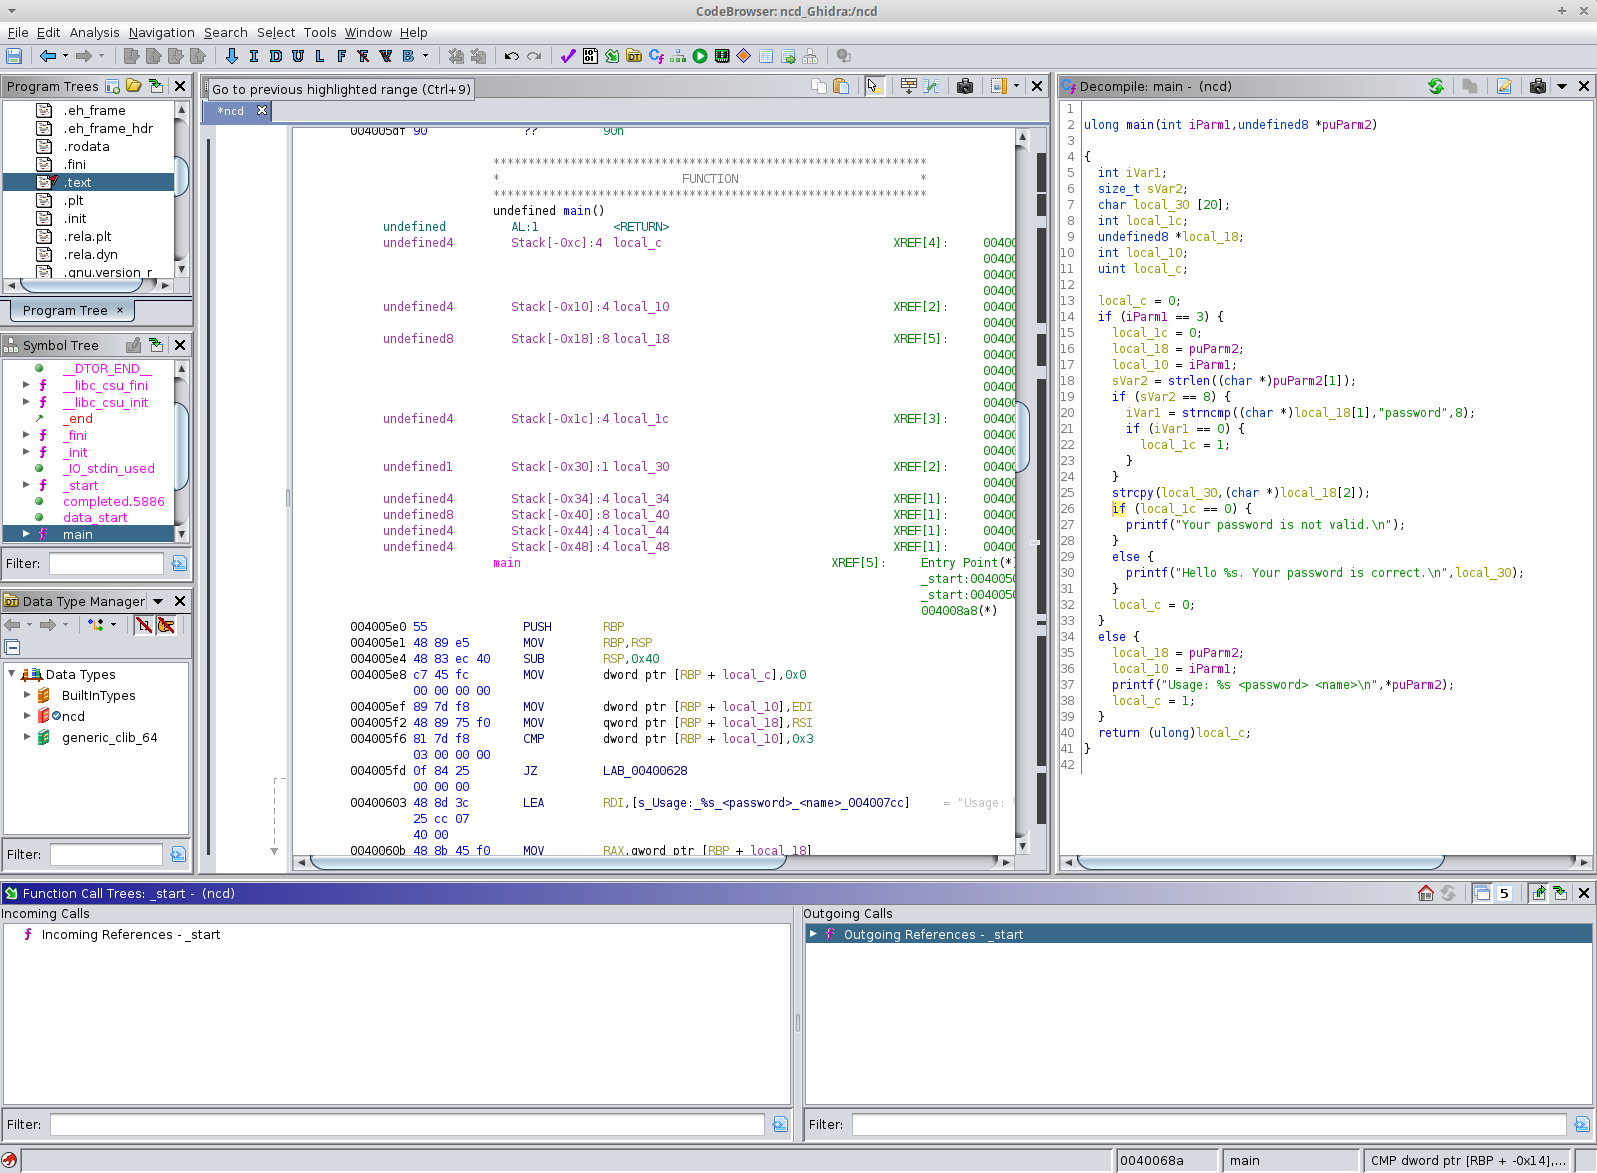
\includegraphics[scale=0.3]{ghidra.png}
		\captionof{figure}{ncd decompiled in Ghidra}
	\end{center}
	
	Nach Schritt 7 erhält man folgenden Code:\\
	
	\begin{lstlisting}[style=CStyle]
		ulong main(int iParm1,undefined8 *puParm2)
		
		{
			int iVar1;
			size_t sVar2;
			char local_30 [20];
			int local_1c;
			undefined8 *local_18;
			int local_10;
			uint local_c;
			
			local_c = 0;
			if (iParm1 == 3) {
				local_1c = 0;
				local_18 = puParm2;
				local_10 = iParm1;
				sVar2 = strlen((char *)puParm2[1]);
				if (sVar2 == 8) {
					iVar1 = strncmp((char *)local_18[1],"password",8);
					if (iVar1 == 0) {
						local_1c = 1;
					}
				}
				strcpy(local_30,(char *)local_18[2]);
				if (local_1c == 0) {
					printf("Your password is not valid.\n");
				}
				else {
					printf("Hello %s. Your password is correct.\n",local_30);
				}
				local_c = 0;
			}
			else {
				local_18 = puParm2;
				local_10 = iParm1;
				printf("Usage: %s <password> <name>\n",*puParm2);
				local_c = 1;
			}
			return (ulong)local_c;
		}
	\end{lstlisting}
	\bigskip
	
	Wählt man als Parameter irgendeinen Namen und als Passwort eine Zeichenfolge, die länger als 20
	Zeichen ist, hält das Programm die Kombination für korrekt.
	\bigskip
	
	Mithilfe des von Ghidra erzeugten C-Codes lässt sich die Funktionsweise des Programms gut nachvollziehen.
	Zu Beginn der 'main' Funktion werden verschiedene lokale Variablen deklariert, für welche 
	der benötigte Speicherplatz auf dem Stack hintereinander reserviert wird.
	Dabei wird der Buffer 'local\textunderscore 30' mit einer Größe von 20 vor dem Integer 'local\textunderscore lc' 
	auf den Stack gelegt.
	Die kritische Stelle ist in Zeile 25, wenn mittels 'strcpy' unser eingegebenes Passwort 
	in den Buffer 'local\textunderscore 30' kopiert werden soll. Da 'strcpy' jedoch kein Bounds-Checking 
	betreibt, überschreiben Passworteingaben, die länger als 20 Zeichen sind, die Variablen, 
	die nach dem Buffer auf dem Stack liegen. In diesem Fall als erstes 'local\textunderscore lc'. 
	'local\textunderscore lc' wird aber in Zeile 26 in einer if-Abfrage dazu genutzt wird, die Korrektheit 
	des Passwortes festzustellen. 
	Ist 'local\textunderscore lc' gleich '0', ist das Passwort falsch. Sonst ist das Passwort richtig. 
	Da durch den Buffer-Overflow 'local\textunderscore lc' mit einem Zeichen überschrieben wurde, 
	welches nicht '0' ist, verhält sich das Programm, als ob das Passwort richtig wäre.
	\bigskip
	
	Eine Möglichkeit, den Angriff zu verhindern, ist, 'strncpy' statt 'strcpy' zu verwenden.
	Alternativ könnte vor dem Aufruf von 'strcpy' die Länge des Strings überprüft werden.
	Ausserdem könnten skalare Variablen vor Buffern deklariert werden, sodass die skalaren 
	Variablen vor den Buffern auf dem Stack liegen und so bei einem Buffer-Overflow keine 
	skalaren Variablen überschrieben werden können. 
	Eine weitere drastische Maßnahme wäre, eine andere Programmiersprache wie Java oder eine 
	interpretierte Sprache zu verwenden, da bei diesen Buffer-Overflows nicht möglich sind.
	\bigskip
	
	Eine Möglichkeit, Buffer-Overflows zu entdecken, ist jede Einagbemöglichkeit mit sehr 
	langen Eingaben zu testen, um einen Buffer-Overflow zu provozieren.
	Eine einfache Möglichkeit, jeden möglichen Buffer-Overflow zu entdecken, gibt es jedoch nicht. 
	Um Programme auf diese Sicherheitslücke zu untersuchen, muss sich jede Verwendung von Buffern 
	genau angeschaut werden. 
	\bigskip
	
	Um zu verhindern, dass ein Angreifer auf den gesamten Arbeitsspeicher zugreifen kann, benutzt 
	Linux zum Beipiel Stack Canaries. Dies sind bestimmte Werte, die auf dem Stack zwischen 
	der Rücksprungadresse und den lokalen Variablen gelegt werden. Diese Werte werden regelmäßig, 
	zum Beispiel vor dem Sprung zur Rücksprungadresse, überprüft. Ist der Wert verändert worden, 
	wird das Programm abgebrochen. SO wird verhindert, dass die Rücksprungadresse verändert wird. 
	Zudem verwendet Linux Paging und Virtual Memory. Der Arbeitsspeicher wird also in Blöcke 
	aufgeteilt, welche eine virtuelle Adresse haben. Versucht ein Programm auf eine Adresse 
	ausserhalb des eigenen Blocks zuzugreifen, entsteht ein Page Fault, sodass das Programm 
	unterbrochen wird. 
	\bigskip

\section*{Teil 2: Format String Attack}
	
	
	\section*{Stichwörter}
	Die folgenden Begriffe sind notwendig für den Versuch zu definieren:
	\begin{itemize}
		\item Format String Attack
		\item printf( ) (die C-Funktion)
	\end{itemize}
	
	Diese, sowie weitere wichtige Begriffe, sollen im Folgenden kurz definiert werden.
	\bigskip
	
	\textbf{Format String Attack} \\
	Format String Attacks bezeichen eine Sicherheitslücke in der Programmierung, bei der Angreifer ein Programm zum Absturz bringen, aber auch potentiell schädlichen Code auszuführen können.
	Es handelt sich hierbei nicht um Sicherheitslücken im klassischen Sinne, viel eher ist es bei Format String Attacks möglich sich Bugs im Code zu Nutze zu machen.
	\bigskip
	
	\textbf{printf( )} \\
	Die printf( )- Funktion ist eine Ausgabefunktion, welche ihren Ursprung in der Programmiersprache C hat. Die Funktion gehört zu den Format Funktionen, welche  eine variable Anzahl von Argumenten als Eingabewerte entgegen nehmen. Einer dieser Werte ist der sogenannte Format String. Dieser ist ein ASCIIZ String, welcher sowohl Text als auch Format Parameter enthält, welche wiederum in der Ausgabe mit einem Wert ersetzt wird. Der Format Parameter gibt an, um welche Art von Ausgabe es sich handelt, beispielsweise Dezimalzahlen oder auch Strings.
	\bigskip
	
	\textbf{Format Funktion} \\
	Eine Format Funktion ist eine ANSI C Funktion, wie \textit{printf( )}, die eine primitive Variable der Programmiersprache in eine, vom Menschen lesbare, String Repräsentation konvertiert.
	\bigskip
	
	\textbf{Format String} \\
	Ein Format String ist ein Argument der Format Funktion und besteht aus einem ASCIIZ String, welcher sowohl Text, als auch Format Parameter enthält.
	\bigskip
	
	\textbf{Format String Parameter} \\
	Ein Format String Parameter definieren den Typ der Umwandlung in einer Format Funktion.
	\bigskip
	
	\textbf{Fragestellung: Wie funktioniert eine Format String Attack grundsätzlich?} \\
	Bei der Format String Attack macht sich der Angreifer eine fehlerhafte Implementation der \textit{printf( )-Funktion} zu Nutze. Wird in dieser kein Format String angegeben, so ist es möglich diese Schwachstelle auszunutzen, indem man einen String übergibt, der gültige \textbf{Format-Parameter} enthält. Diese werden dann als \textit{Format String} interpretiert und ausgeführt, wodurch vom Speicher gelesen wird, was der Angreifer schadhaft ausnutzen kann. Die \textit{Format Funktion} ließt dann einfach die nächsten Daten des Speichers, wodurch es zum Kontrollverlust über den Prozess kommen kann.
	\bigskip
	
	Um den zweiten Teil des Versuches durchzuführen, haben wir folgende Schritte durchgeführt:
	
	\begin{enumerate}
		\item Herunterladen des C-Programms fmtstr.c
		\item Kompilieren des C-Programms fmtstr.c mittels gcc $\rightarrow$ führt zu zwei Warnings, aber zu keinem Error:
			\begin{center}
			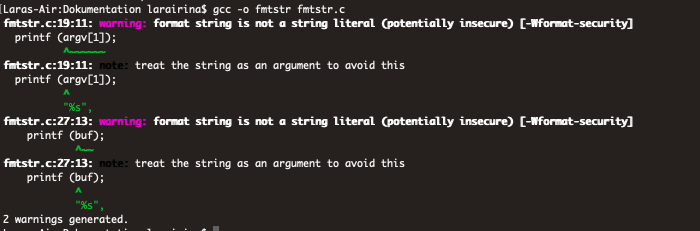
\includegraphics[scale=0.3]{compilation.png}
			\captionof{figure}{Kompilieren des Quellcodes}
			\end{center}
		\item Einfaches Ausführen des Programms ohne Kommandozeilenargumente führt zu folgender Ausgabe:
		\begin{center}
			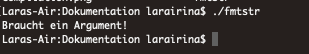
\includegraphics[scale=0.8]{ohneCmdln.png}
			\captionof{figure}{Ausführen des Quellcodes}
		\end{center}
		\item Durch Eingabe zur Laufzeit des unveränderten Programms soll der Wert der Variable \textbf{x} verändert werden  $\rightarrow$ Eingabe: "\%x \%x \%x \%x \%x \%x \%x \%x \%n"
		\item Das Vorzeichen der Variable \textbf{x} soll nun durch eine weitere Eingabe umgedreht werden $\rightarrow$ Eingabe "\%155x \%9\$n"
	\end{enumerate}

	Durch Veränderung der Print-Anweisung in Zeile 30 (siehe Figure 3) ist es einem Angreifer nun nicht mehr möglich dem Compiler einen eigenen Format String zu übergeben und ein Angriff wird so verhindert, da die Variable \textbf{buf} nun nur noch als String, also als Daten-Parameter, interpretiert wird.

\begin{center}
	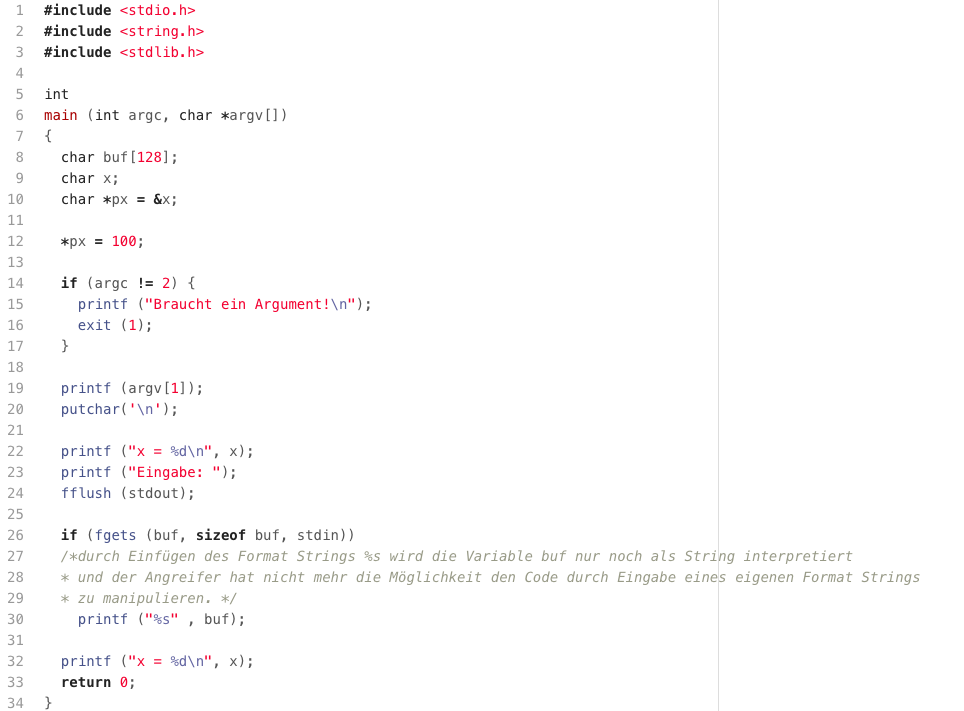
\includegraphics[scale=0.3]{betterCode.png}
	\captionof{figure}{Verbesserter Quellcode}
\end{center}
	
	\section*{Fragen}
	\textbf{Wie kann ein*e Programmierer*in einfach dafür Sorge tragen, dass Format String Angriffe nicht mehr möglich (oder zumindest erheblich erschwert) sind?} \\
	Eine einfache Möglichkeit Format String Angriffe zu verhindern oder erschweren ist die Analyse des Programmcodes. Wird einer Format Funktion wie \textit{printf( )} nur ein Wert übergeben, so kann man davon ausgehen, dass hier ein Angriff möglich ist. Schwachstellen werden so effizient vermieden und die Analyse lässt sich auch automatisiert ausführen. Trotz aller Einfachheit ist hierbei zu beachten, dass ausreichende Programmierkenntnisse notwendig sind um Patches zu erstellen und Quellcodes zur manuellen Analyse häufig zu komplex sind. 
	\bigskip

	Eine weitere Möglichkeit zur Prävention ist das Prüfen auf Speichergrenzen von Variablen während der Programmausführung. So können Buffer Overflows während der Laufzeit erkannt und Angriffe vermieden werden. Um diese Maßnahme anwenden zu können, muss der Quellcode jedoch überarbeitet werden und auch die Performanz kann darunter leiden.
	\bigskip
	
	\textbf{Wie lässt sich einfach herausfinden, ob ein derartiger Angriff vermutlich möglich ist?} \\
	Durch eine Analyse des Quelltextes lässt sich einfach herausfinden, ob ein Format String Angriff möglich ist. Hierbei gilt es herauszufinden, wie viele Werte einer Funktion der printf( )-Familie übergeben werden. Bekommt die Funktion nur einen Wert übergeben, so wird dies ials eine Art benutzerdefiniertes Format interpretiert. Werden jedoch mehr als ein Wert übergeben, so ist davon auszugehen, dass die Format Strings fest vorgegeben sind und ein derartiger Angriff nicht möglich ist. 
	\bigskip
	
	
\end{document}